\section{Experimental Validation}
\label{S:Exp}

In this section we present how the data set was generated, the time it takes to map 95\% of the environment, and a comparison between using Howard's algorithm and the independently sampled algorithm.  




\subsection{The Data Set}
\label{S:Exp:DataSet}

The data set consists of PAS triple $(\textbf{x}^{R(i)}_t,u^{R(i)}_t,z^{R(i)}_t)$, where $R$ denotes the robot ID, and $t$ denotes the time.  The pose, $\textbf{x}^{(i)}_t$, is comprised of the $x_t^R$-$y^R_t$ position, as well as the orientation $\theta^R_t$.  The input, $u^R_t$, is composed of the position deflection, $\delta^R_t$, and the angular deflection, $\omega_t$.  Finally, the measurements, $z^R_t$, contains scan data for rays cast out at $1^\circ$ intervals from $[-90^\circ,90^\circ]$, to simulate a laser scan.  

To obtain the measurements a binary map, $I$, and the ray-circle intersection algorithm.

\subsubsection{Ray-Circle Intersection}

The scan data is constructed using ray-circle intersection of a binary image, $I$ (like that of Fig. \ref{subfig:Enc} without the paths).  The idea of ray-circle intersection is to find all the object pixels within a region of interest (ROI), in this case the shaded pixels in the semi-circle, $I_{semi}$, as seen in Fig. \ref{subfig:raycirc}, 
\begin{equation}
I_{semi}=\left\{I_{xy}\in I |\  ||I_{xy}-I_{\textbf{x}_t^R}||_2^2<r^2 \right\},
\label{eq:Isemi}
\end{equation}
where $I_{\textbf{x}_t^R}$ is the position of the robot $R$ in the map, and $I_{xy}$ denotes the pixels $(x,y)$.

Then $I_{semi}$ is intersected with the object, $I_{obj}=\{I_{xy}\in I | \ I_{xy}=1\}$ (the filled squares in Fig. \ref{subfig:raycirc}, to get $I_{filled}$.  A ray is then defined by 
\begin{equation}
\textbf{v}_k=\begin{bmatrix}
I_{x_t^R}+r_k^j \cos(\phi_k)\\
I_{y_t^R}+r_k^j \sin(\phi_k)\\
\end{bmatrix}, 
\label{eq:ray}
\end{equation}
where $r_k^j>0$ is some partitioning of the length of the ray up to the maximum range of the sensor.  This ray is intersected with $I_{filled}$ to get $I_{ray}$ (colored in orange in Fig. \ref{subfig:raycirc}).  Finally, the minimum distance to the object, $r_{k}^*$ , is selected (the $r_k^j$ corresponding the blue square in Fig. \ref{subfig:rstar}) to get the distance measurement $z_t^{R,k}$ of the object to the robot.  

\begin{equation}
r_k^*=\min_{j} r_{k}^j
\end{equation}


\begin{figure}[ht]
\centering
\subfigure[$I_{filled}$ and the intersection with the ray $\textbf{v}_k$.]{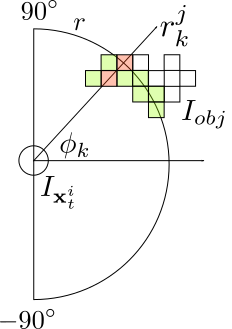
\includegraphics[height=4cm]{../FinalFigures/RayCircleIntersection1}\label{subfig:raycirc}}
\subfigure[The selection of $r_k^*$.]{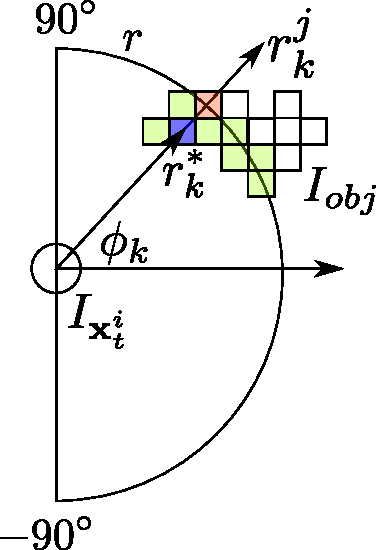
\includegraphics[height=4cm]{../FinalFigures/RayCircleIntersection}\label{subfig:rstar}}
\caption{Visualization of ray-circle intersection algorithm.}
\label{fig:raycirc}
\end{figure}

To obtain experimental-like data, we introduce zero mean, additive Gaussian noise with variance $Q$ to $z_t^{R,k}$ to get noisy measurements $\hat{z}_t^{R,k}$:
\begin{equation}
\hat{z}_t^{R,k}=z_t^{R,k}+\mathcal{N}(0,Q).
\end{equation}

\subsubsection{Wall Following}

For our coordination, we use wall following to search the environment.  The specifics of this implementation are: wall following is turned on when $t\in[50,200]$, each robot is equipped with a parity bit to ensure that some robots move in opposite directions, and if the robot happens to get stuck in a loop, wall following will temporarily turn off.

Using wall following to search the environment led to the choice of the odometry motion model, because wall following can be easily implemented in conjunction with scan data obtained using ray-circle intersection.


\subsubsection{The Odometry Motion Model}

The motion model used was a classic odometry motion model.  
\begin{equation}
\begin{bmatrix}
x_{t}\\
y_{t}\\
\theta_{t}
\end{bmatrix}=\begin{bmatrix}
x_{t-1}\\
y_{t-1}\\
\theta_{t-1}
\end{bmatrix}+\begin{bmatrix}
\hat{\delta}_{t-1}  \cos(\theta_t+\hat{\omega}_t)\\
\hat{\delta}_{t-1}\sin(\theta_t+\hat{\omega}_t)\\
\hat{\omega}_{t-1}
\end{bmatrix},
\label{eq:OdometryMotion}
\end{equation}
where
\begin{eqnarray}
\hat{\delta}_{t-1}&=&\delta_{t-1}-\mathcal{N}(0,\alpha_1\delta_{t-1}^2+\alpha_2\omega_{t-1}^2)\\
\hat{\omega}_{t-1}&=&\omega_{t-1}-\mathcal{N}(0,\alpha_3\delta_{t-1}^2+\alpha_4\omega_{t-1}^2).
\end{eqnarray}

This results in the reverse odometry model:
\begin{equation}
\begin{bmatrix}
x_{t-1}\\
y_{t-1}\\
\theta_{t-1}
\end{bmatrix}=\begin{bmatrix}
x_{t}\\
y_{t}\\
\theta_{t}
\end{bmatrix}-\begin{bmatrix}
\hat{\delta}_t  \cos(\theta_t-\hat{\omega}_{t-1})\\
\hat{\delta}_{t}\sin(\theta_t-\hat{\omega}_{t-1})\\
\hat{\omega}_{t-1}
\end{bmatrix}.
\label{eq:ReverseOdometryMotion}
\end{equation}

With these motion models we may now discuss how the robot encounters and determines relative poses.  


\subsubsection{Encounter Detection and Relative Pose}

In place of using a hypothetical camera to determine if robot encounters occur, we use the ray-circle intersection algorithm.  We treat each robot as an object in the binary image, $I$, and if a $(r_k^*,\phi_k)$ is found to coincide with an added robot, and encounter is declared and a relative pose is calculated is calculated from \eqref{eq:relpose}.



\subsubsection{The Environment, Robot Trajectories, and Encounters}

  Fig. \ref{subfig:Encvst} shows at what time a robot encountered another, note: only the first encounter is used.

Fig. \ref{subfig:Enc} shows the binary map of the environment, the paths each robot took (solid lines), the point when a robot encounter occurred (dashed gray lines), where the first encounter occurred (thick grey line), the particles at the final time step (attached to the solid lines), and the global pose (corresponding circles) for comparison.

For ease of use, we will set Robot 1's initial pose as the global frame's origin.  

\begin{figure}[ht]
\centering
\subfigure[Robot encounters versus time.]{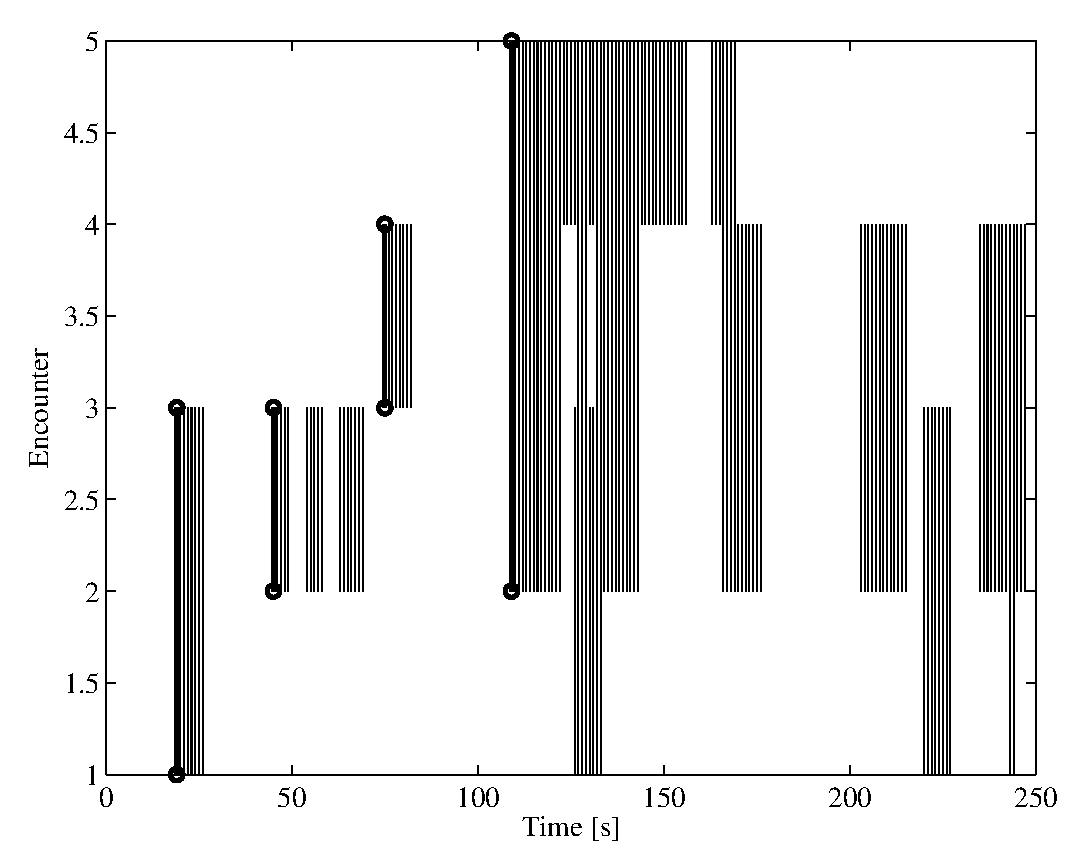
\includegraphics[width=\columnwidth]{../FinalFigures/EncountersTimes}\label{subfig:Encvst}}
\subfigure[The test geometry, robot paths (colored lines), and encounters (dashed gray lines).]{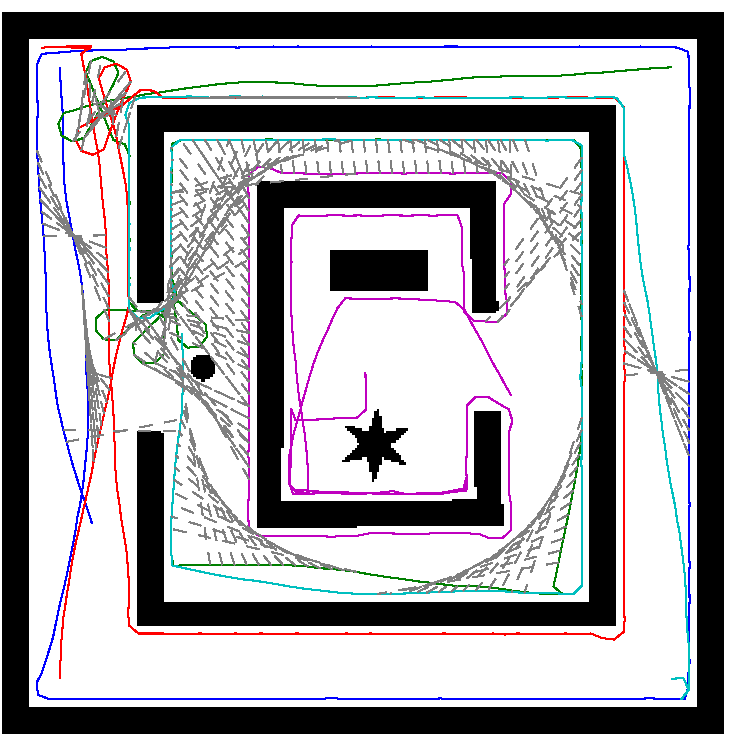
\includegraphics[width=\columnwidth]{../FinalFigures/Encounters}\label{subfig:Enc}}
\caption{Environment geometry, robot paths, and encounters.}
\label{fig:EnvEnc}
\end{figure}



\subsection{Timing}
\label{S:Exp:Timing}

One of the primary motivations for using MRSLAM is to decrease the amount of time it takes to complete the mapping objective.  In this section we demonstrate that generally speaking the time it takes to map an environment decreases with the number of robots.  

To present the time it takes to map the environment, we must first define what we mean by mapping the environment.  When we say that we have mapped an environment, we mean that we have created an occupancy grid, $J$, that matches the outermost black edges of Fig. \ref{subfig:knownpose} using a perfect sensor/actuator.  

To obtain the edges of the binary map, $I$, we use morphological erosion to obtain $\tilde{I}$:
\begin{equation}
\tilde{I}=I\ominus \begin{bmatrix}
1 & 1 & 1 \\
1 & 1 & 1 \\
1 & 1 & 1
\end{bmatrix},
\end{equation}
then padding $\tilde{I}$ with zeroes, we take the exclusive or of $I$ and $\tilde{I}$ to $I_{edge}$:
\begin{equation}
I_{edge}=(\tilde{I}\wedge \neg I)\vee (\neg \tilde{I}\wedge I).
\end{equation}
Then we define the percent mapped as
\begin{equation}
\zeta =\frac{\sum_{x,y}I_{edge}\wedge J}{\sum_{x,y}I_{edge}},
\end{equation}
and when $\zeta\geq 0.95$, we say that the environment has been mapped.

Using 100 different trials, Table \ref{table:timing} provides the average amount of time it took to map 95\% of the environment using different number of robots.  To note is that the averages do tend to decrease as expected.  However, it should be noted that there is a large degree of uncertainty, at least until we get beyond 7 robots.  

\begin{table}
\centering
\caption{Time to map 95\% of the environment.}
\label{table:timing}
\begin{tabular}{c|c|c|c|c}
\hline
\hline
\# Robots & Mean & Std  & Max & Min \\
\hline
1 &  501.5185  &  99.4  & 684  & 341\\
\hline
2 &  357.3182  & 170.8  & 654  & 162\\
\hline
3 & 201.8646   & 92.4  & 549  & 122\\
\hline
4 &  332  & 179.2 & 681  & 140\\
\hline
5 &  212.8191  & 113.4  & 523  & 117\\
\hline
6  & 242.4524  & 120.7  & 594  & 100\\
\hline
7  & 262.9425  & 134.3  & 681  &  79\\
\hline
8  &  74.1717  &  20.1 &  150  & 55\\
\hline
9  &  72.0101  &  27.4  & 257   & 54\\
\hline
10  &  56.9600  &   6.3  &  91  &  48\\
\hline
\hline
\end{tabular}
\end{table}



\subsection{The Results}
\label{S:Exp:Results}

\newcommand{\multiplier}{7.25cm}
\begin{figure*}[th]
\centering
\subfigure[Pure Odometry, high noise.]{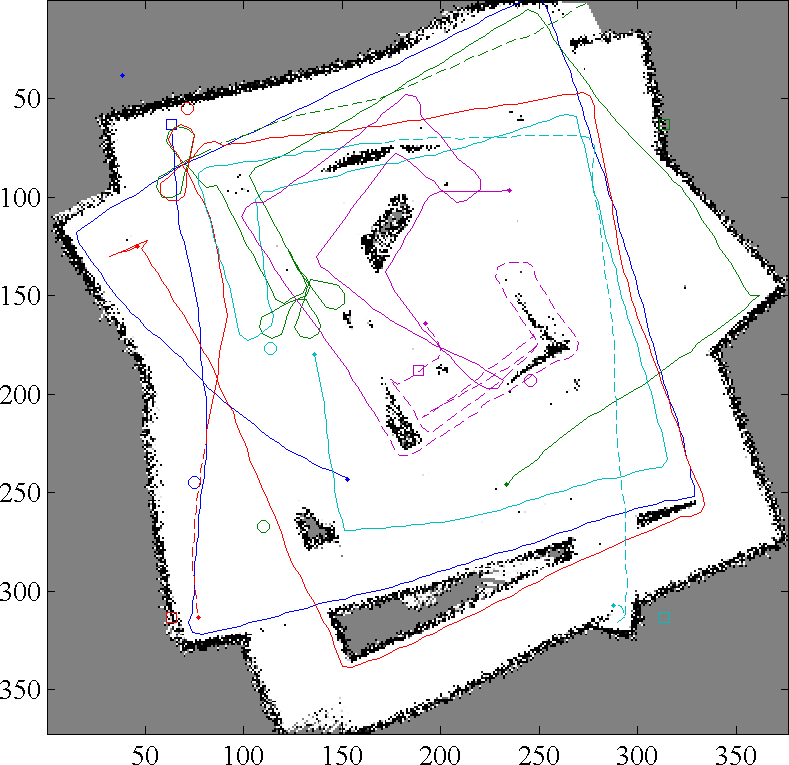
\includegraphics[width=\multiplier]{../FinalFigures/PureOdometry}\label{subfig:pureodom}}
\subfigure[Known Poses]{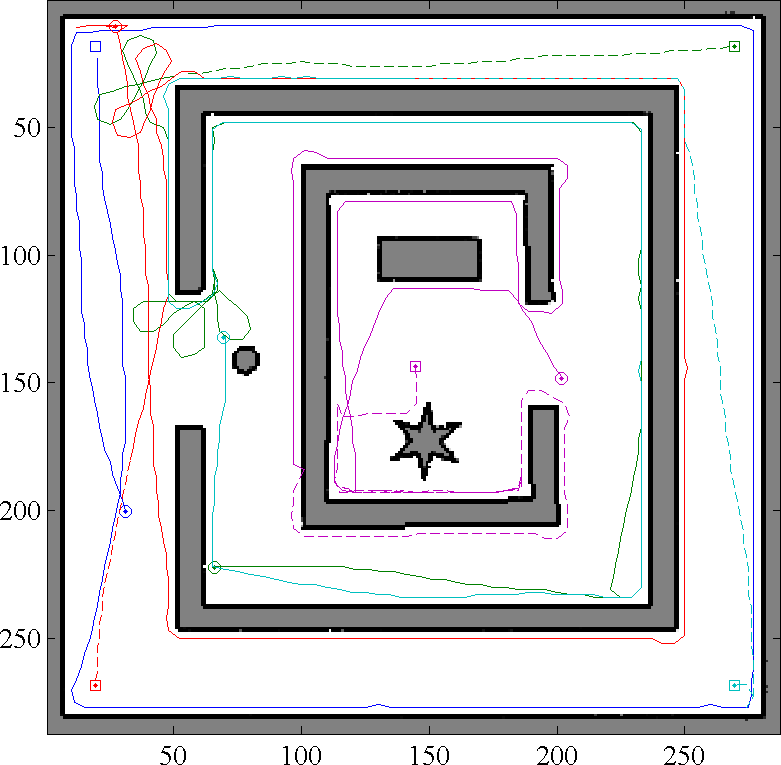
\includegraphics[width=\multiplier]{../FinalFigures/KnownPoses}\label{subfig:knownpose}}\\
\subfigure[Howard Implementation: Unknown Poses, low noise.]{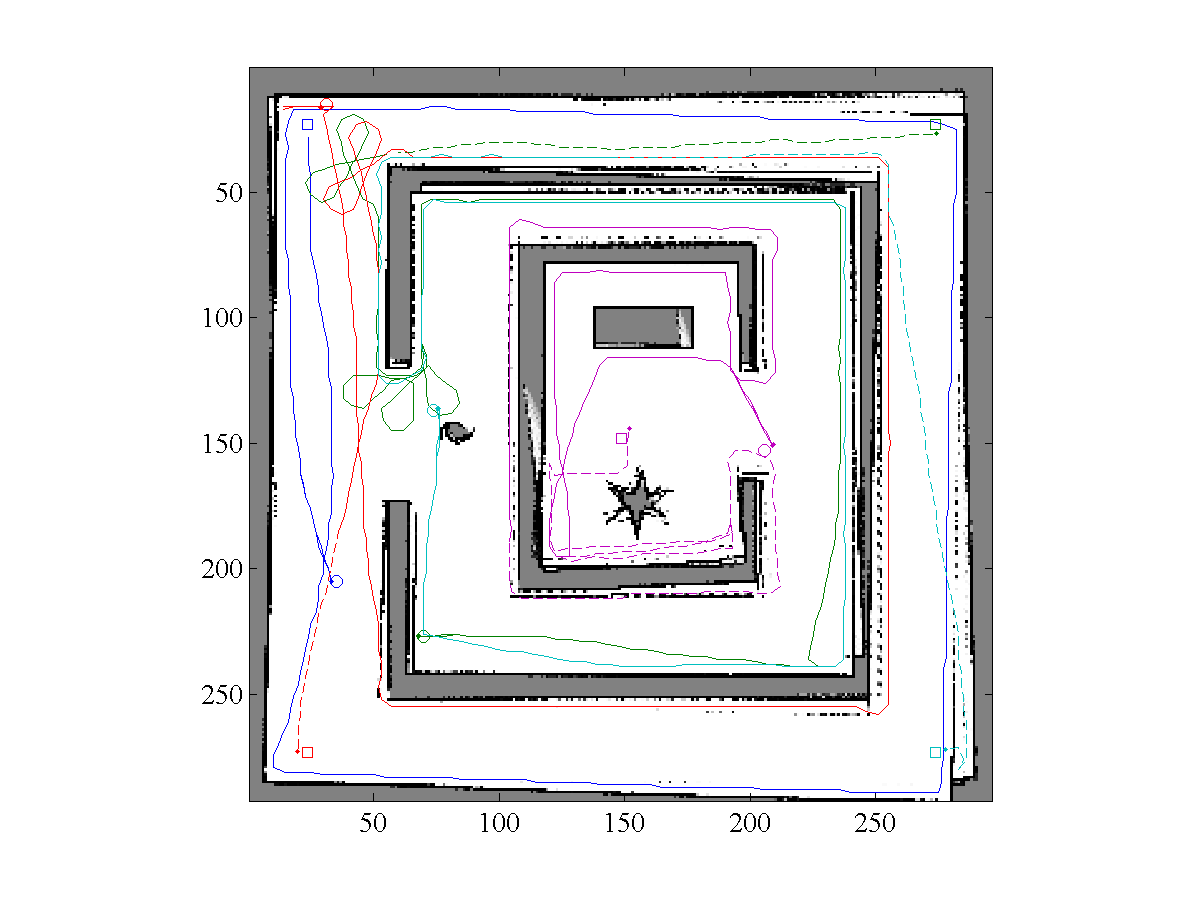
\includegraphics[width=\multiplier]{../FinalFigures/HowardLowNoise}\label{subfig:HowardLow}}
\subfigure[Proposed Implementation: Unknown Poses, low noise.]{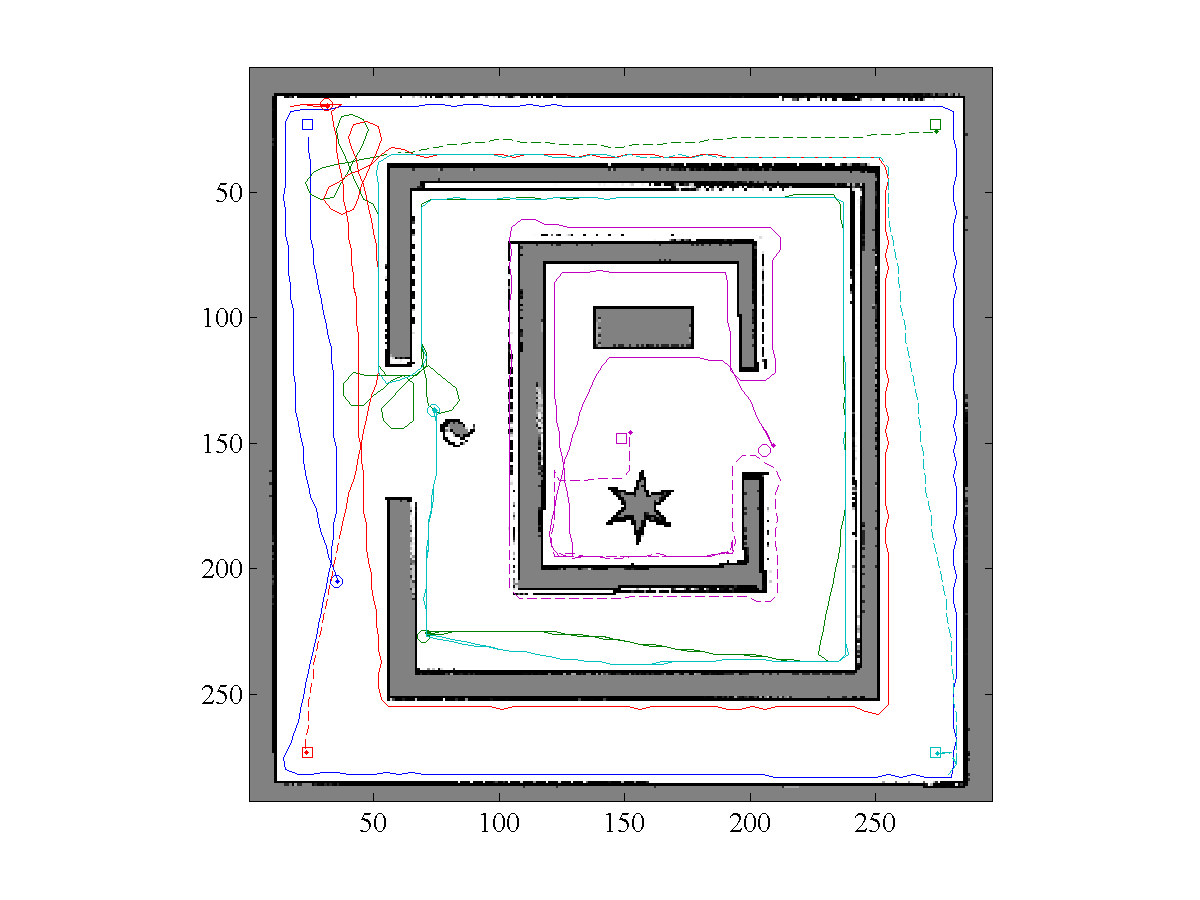
\includegraphics[width=\multiplier]{../FinalFigures/OursLowNoise}\label{subfig:OurLow}}\\
\subfigure[Howard Implementation: Unknown Poses, High noise.]{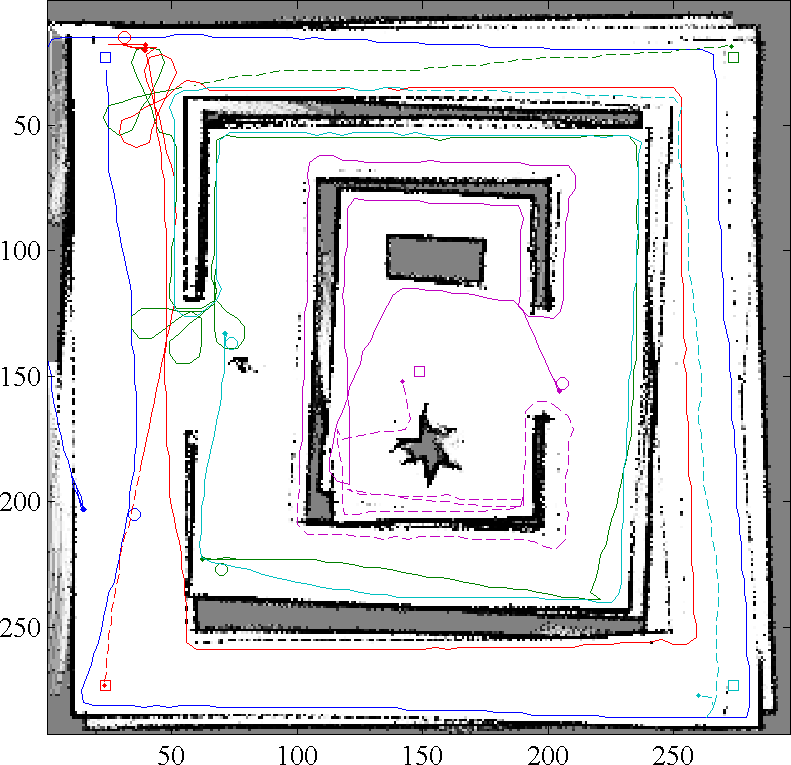
\includegraphics[width=\multiplier]{../FinalFigures/HowardHighNoise}\label{subfig:HowardHigh}}
\subfigure[Proposed Implementation: Unknown Poses, High noise.]{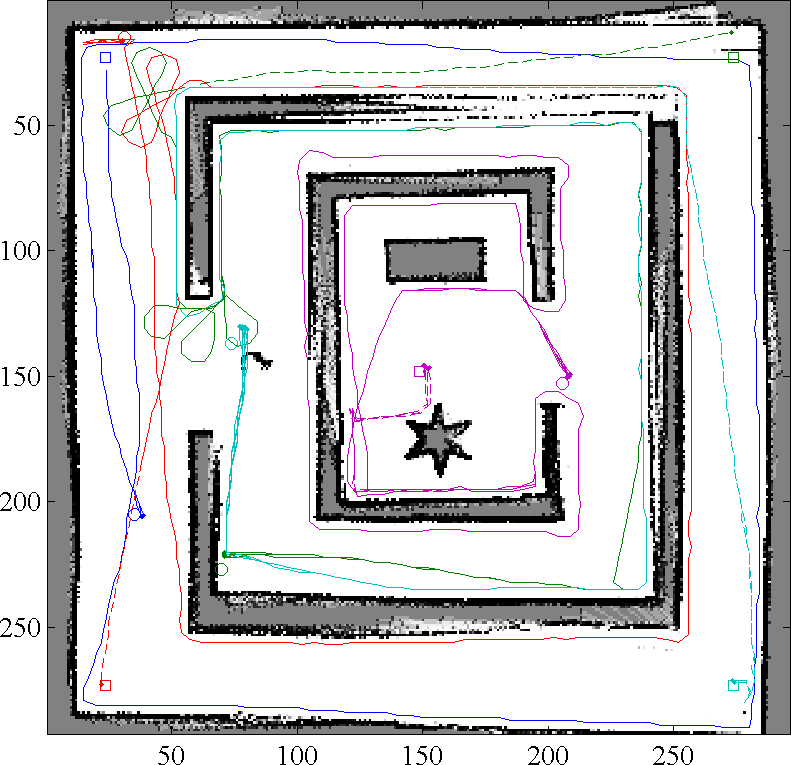
\includegraphics[width=\multiplier]{../FinalFigures/OursHighNoise}\label{subfig:OurHigh}}
\caption{Comparison between Howard's implementation and the proposed implementation.}
\label{fig:Comp}
\end{figure*}

From Table \ref{table:timing} we see that there is a large drop-off when we increase the number of robots from 2$\rightarrow$3, 4$\rightarrow$5, and 7$\rightarrow$8.  Despite it has the highest average time, 5 robots nicely conveys the complexity that can be achieved; as such, 5 robots, each with 30 particles, will be used to highlight the improvement of the independently sampled algorithm over Howard's using a 250 second simulation.  

To compare the two algorithms, we use two sets of sensor/actuator data: a low noise set and a high noise set. 
\begin{description}
\item[\textbf{Low}] The low noise set perturbs the actuator input by $\mathcal{N}(0,0.1)\ [m]$ on $\delta_t^{R}$, $\mathcal{N}(0,0.01)\ [m]$ on $\omega_t^{R}$, and $\mathcal{N}(0,0.5)\ [m]$ on $z_t^{R,k}$.  
\item[\textbf{High}] The high noise set perturbs the actuator input by $\mathcal{N}(0,1)\ [m]$ on $\delta_t^{R}$, $\mathcal{N}(0,0.1)\ [m]$ on $\omega_t^{R}$, and $\mathcal{N}(0,1.5)\ [m]$ on $z_t^{R,k}$.
\end{description}

The qualitative results are presented in Fig. \ref{fig:Comp}.  Fig. \ref{subfig:pureodom} provides the occupancy grid if pure odometry was used, to contrast the poor performance the occupancy grid using known poses is given in Fig. \ref{subfig:knownpose}.

For Fig. \ref{subfig:HowardLow} and \ref{subfig:HowardHigh}, the solid and dashed line represent the best estimated trajectory in the causal and acausal directions.  Whereas, for Fig. \ref{subfig:OurLow} and \ref{subfig:OurHigh}, the solid and dashed lines represent the best estimated path for the causal and acausal data, respectively.

Fig. \ref{subfig:HowardLow}-\ref{subfig:OurHigh} provide the comparison between Howard's and the proposed algorithm.  Comparing Fig. \ref{subfig:HowardLow} and \ref{subfig:OurLow}, it is easy to see that the proposed implementation is almost as good as the occupancy grid with known poses (Fig. \ref{subfig:knownpose}).  Even in the high noise case, Fig. \ref{subfig:HowardHigh} and \ref{subfig:OurHigh}, we see less error with the independently sampled algorithm.  

Over the number of particles, we define the minimum sum of squares error (a.k.a. the least absolute deviation error):
\begin{equation}
\varepsilon=\min_{k\in\{1,\cdots,n\}}\sqrt{\sum_{R=1}^{M} ||\textbf{x}_{t}^R-\hat{\textbf{x}}^{R,k}_{t}||^2_2}
\end{equation}
where $n$ is the number of particles, $M$ is the number of robots, and $\textbf{x}_t^R$ is the known pose, $\hat{\textbf{x}}^{R,k}_{t}$ is pose of particle $k$ in the global frame.  Using this measure, Fig. \ref{fig:minsumerr} quantitatively demonstrates that the independently sampled algorithm provides a better estimate of the pose for nearly all time instants.  Note: for the first 100 seconds, both techniques have the same error, but for the high noise case, the independently sampled algorithm dominates with less than half the error of Howard's algorithm.  Enclosed are videos highlighting Fig. \ref{fig:Comp}.




\begin{figure}[h]
\centering
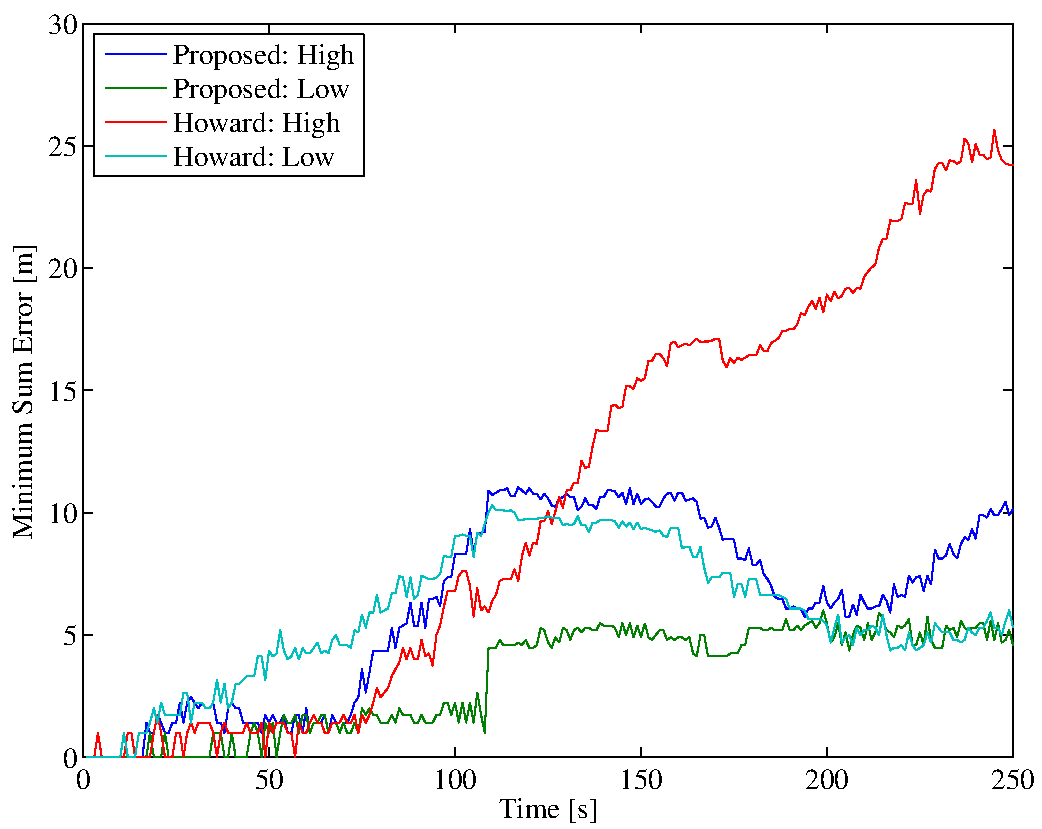
\includegraphics[width=\columnwidth]{../FinalFigures/MinSumError}
\caption{Minimum sum square error versus time.}
\label{fig:minsumerr}
\end{figure}